\chapter[Structure-function mapping pipeline]{Structure-function mapping of mitochondrial membrane potential onto 3D mitochondrial networks}\label{ch:two}
\vfill
Portions of this chapter were published in \emph{M. P. Viana, S. Lim, and S. M. Rafelski, “Chapter 6 - Quantifying mitochondrial content in living cells,” in Methods in Cell Biology, vol. 125 of Biophysical Methods in Cell Biology, pp. 77–93, Academic Press, 2015}.
\section{Introduction}
Mitochondria in yeast form a three-dimensional network structure localized to the cortical periphery of the cell. This network displays a dynamic morphology that changes in response to the metabolic state of the cell. Many groups have therefore studied the structure of the mitochondrial network as they could correlate metabolic, genetic and biochemical data with the morphological changes to the organism. However, a significant challenge has been to quantify automatically these structural features with functional state in a rigorous an unbiased manner. Ideally an automated structure-function mapping pipeline should be able to provide spatial information that enables one to analyze the distribution of the functional marker down to the level of individual tubules within the network. However as we shall detail in this chapter, such a pipeline has been lacking in the field.

Since the 1970's, effort had been made to characterize the overall structure of the entire mitochondrial network using serial thin sections of chemically fixed cells \cite{hoffmann_mitochondrion_1973}. Indeed the first computer aided visualization of the mitochondrial network was done in 1979 based on these thin section data \cite{stevens_mitochondrial_1981}. This was a laborious method which involved digitizing hand tracings of the mitochondrial network. With the advent of a matrix targeted fluorescent protein (FP) marker, live cell 3D imaging of the mitochondrial network was demonstrated for the first time by \cite{nunnari_mitochondrial_1997}. Since then further improvements have come from higher optical resolution (confocal and super resolution microscopy \cite{egner_fast_2002}) together with advances in image processing algorithms of the network itself. 

It was not long before the technique of using fluorescent imaging of live cells was used to study mitochondrial structure and their relationship with functional state changes. Although done in mammalian cells, the work by \cite{koopman_simultaneous_2006} was particularly unique for adopting a quantitative approach to obtaining measurements of mitochondrial morphology and function. They used a lipophilic cationic dye (Rhodamine 123) which accumulates in the mitochondria in a membrane potential ΔΨ dependent manner to label the mitochondrial structure and simultaneously ΔΨ. This study was noteworthy for using quantitative descriptors for mitochondrial morphology, for example rather than using qualitative descriptions of mitochondrial shapes such as 'tubular', 'fragmented' or 'swollen' which was typical for that time \cite{jakobs_spatial_2003,sesaki_division_1999}, they used objective shape parameters such as aspect ratio, perimeter, area and form factor. However their study only showed bulk measurements of ΔΨ and did not actually map local ΔΨ variations within network. Another shortcoming was their segmentation methods for mitochondria was relatively simple, because they were working with flat, 2 dimensional fibroblast cells. 

A major shortcoming of the above study and others \cite{mcfaline-figueroa_mitochondrial_2011} is that they only used a single reporter for mitochondrial structure and function. This means that they could not label the mitochondrial structure in a manner that was independent of the functional state of the network. The lack of a dual reporter system also results in false variability artifacts in the functional channel, which are detailed in \fref{sec:artifacts}. The use of a dual reporter system is critical to control for false variability in the functional channel, and more groups have started to implement normalization methods to control for this false variability \cite{gerstenberger_heterogeneity_2012,vowinckel_mitoloc:_2015,wikstrom_-cell_2007}

Perhaps even more important is a reliable, validated approach to segment the 3D mitochondrial network. For example one group quantified redox state and reactive oxygen species (ROS) levels in yeast mitochondrial networks using an image intensity based segmentation of the network \cite{mcfaline-figueroa_mitochondrial_2011}. However intensity based segmentation is very sensitive to thresholding parameters and their data does not indicate how their segmentation was validated nor did it give any indication that they could obtain three dimensional topological data from their segmentation method. Perhaps the closest to an ideal structure function mapping approach was in a recent study by Vowinckel et al. \cite{vowinckel_mitoloc:_2015}. In this study they used a dual reporter system to co-label yeast mitochondrial structure using a matrix targeted FP together with a respiratory chain associated protein FP whose import is membrane potential dependent. They presented a validated mitochondria segmentation software (Mitoloc) to quantify structure and function in yeast mitochondria. However their quantification methods for mitochondrial morphology focused more on shape parameters that distinguish the 'fragmentation', 'condensation' or 'tubular' state of the network. In other words they did not study the connections within the network itself, but rather overall parameters for describing the morphology of the entire network.

We present a completely open-sourced pipeline for multi-scale, quantitative analysis of structure and function in yeast mitochondrial networks. Our approach combines the outputs of MitoGraph v2.0 \cite{viana_chapter_2015}, a mitochondrial segmentation and skeletonization software developed in the Rafelski lab with additional algorithms to map a functional dye ΔΨ onto mitochondrial networks expressing a matrix targeted FP.
\subsection{Development of a structure function mapping pipeline}
MitoGraph v2.0 is a fully validated software developed in the Rafelski lab by M.Viana. It uses non-intensity based image processing techniques for accurate (85\%) and reproducible (96.7\%) segmentation of mitochondrial network in yeast \cite{viana_chapter_2015} . In this project, we used the outputs of MitoGraph v2.0 skeletonization routine to obtain spatial information of mitochondrial networks labeled with a matrix targeted FP. We then developed a voxel by voxel colocalization pipeline to map a channel for a dye that labels ΔΨ distribution along the network. We used a lipophilic cationic dye, 3,3$'$-dihexyloxacarbocyanine iodide (DiOC$_6$) that accumulates in the matrix in a ΔΨ dependent manner. DiOC$_6$ is a popular choice for labeling ΔΨ in yeast studies, as it falls under a class of lipophilic dyes that accumulate according to the Nernst equation:
\begin{equation}
\mupDelta\mupPsi =  \frac{RT}{zF}\: ln\frac {[\mathrm{ion_{mito}}]}{[\mathrm{ion_{cyto}}]}
\end{equation}
Where $R$ is the universal gas constant, $T$ is the absolute temperature, $z$ is the charge of the cation and $F$ is Faraday constant
\section{Materials and Methods}\label{sec:MM2}
\subsection{Spinning disk microscopy platform}
 All images in this thesis were obtained using a spinning disk confocal microscope with a motorized stage to enable live cell three dimensional microscopy as shown in \Fref{fig:optics}. The microscope chassis (Nikon Eclipse Ti) was paired with a Yokogawa CSUX spinning disk head. The objective was an oil immersion 100× with (NA 1.49) with a correction collar.

Excitation source were from two Coherent Optically Pumped Semiconductor Laser modules at \SI{488}{\nm}/\SI{561}{\nm} synchronized with the camera using custom TTL hardware (SolamereTech). Laser switching was achieved via an acousto-optic tunable filter (AOTF, Solameretech) which enables near instantaneous switching times (<0.1 ms). The dichroic and emission filter was a multiband filter set from Chroma (TRF89901-EM) with passbands at DAPI/GFP/RFP/Cy5 emission spectrum.
An ASI (Eugene, OR) piezoelectric focus and motorized stage enabled automated stack acquisition. Acquisition software was via MicroManager ImageAcquistion software (v 1.4.17).  All imaging was done at 30°C via a temperature controlled housing over the chassis (inVivo Scientific). The camera was a low noise Hamamatsu EMCCD (C9100-23B) camera air cooled to -65°C with a 512×512 pixels imaging back-thinned CCD enabling high quantum efficiency of up to 90\%, with a fastest readout speed of 32 frames/sec at 1× binning. The entire platform rests on a vibration isolating table (TMC, Ametek MA).
%
\begin{figure}[htp]
	\centering
    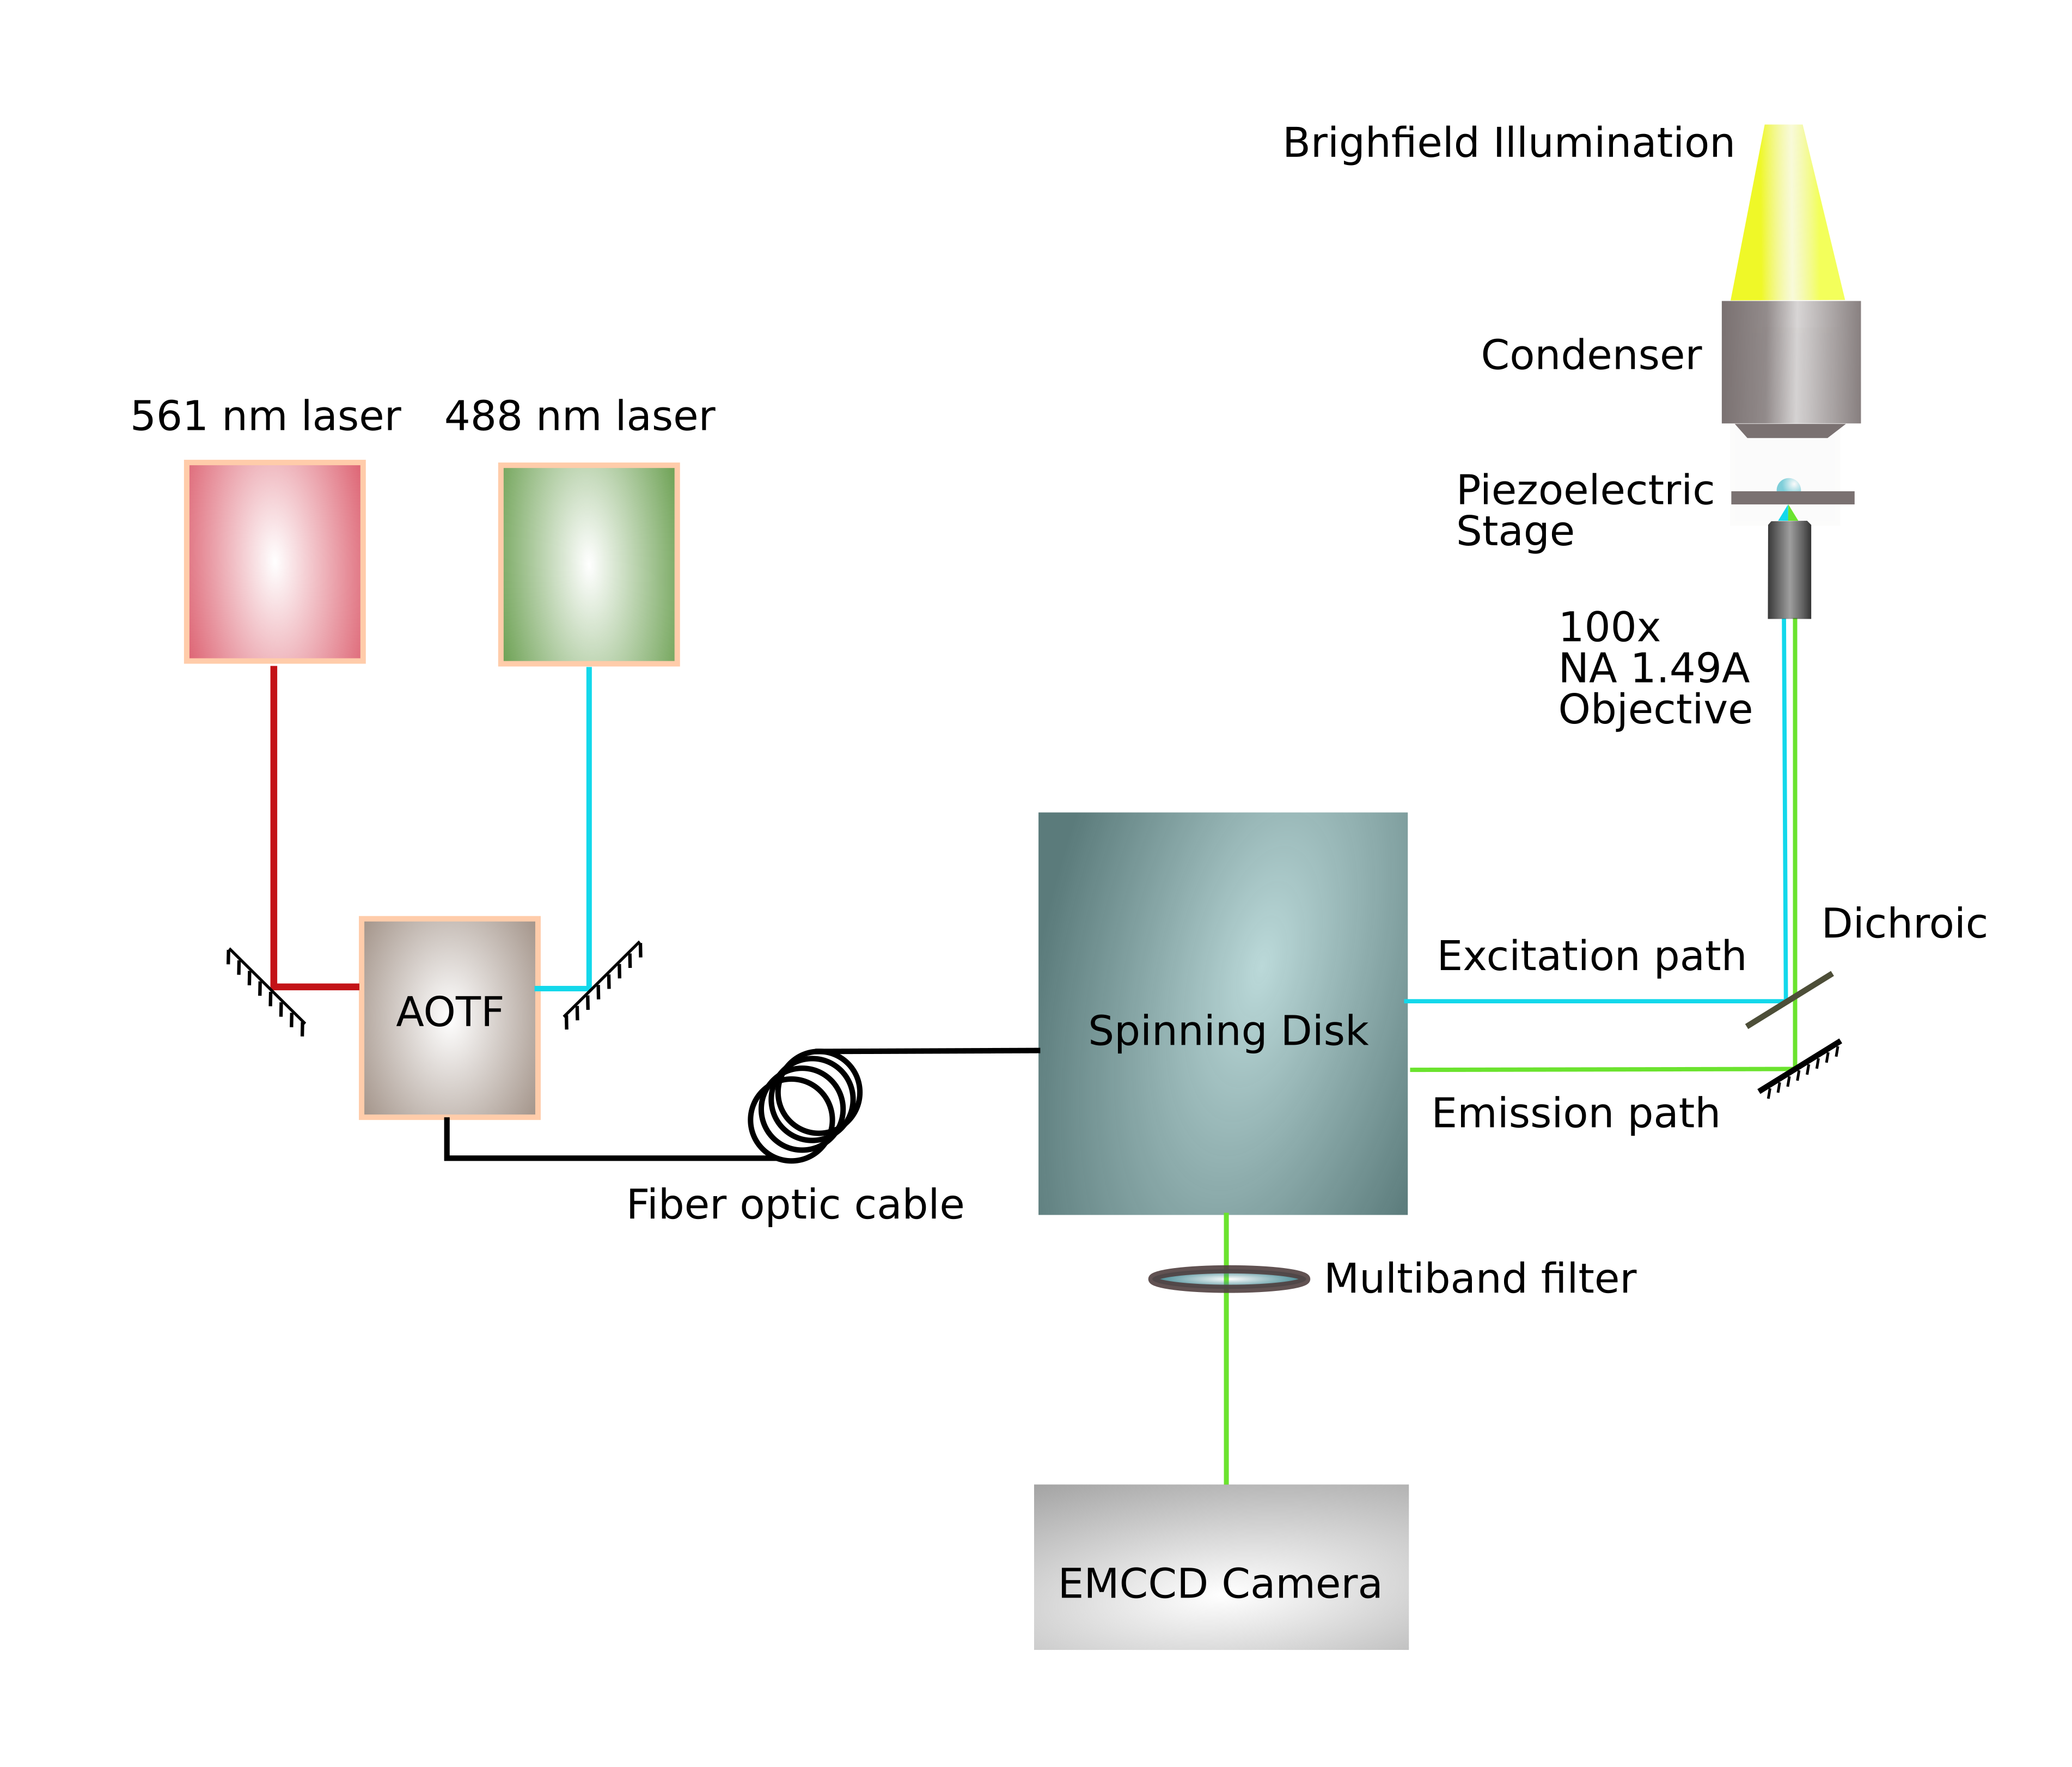
\includegraphics[width=\textwidth]{optics}
    \caption{Schematic diagram of the spinning disk microscope platform.}\label{fig:optics}
\end{figure}
%
\subsection{Strain construction for visualization of matrix structure}\label{sec:strain}
The original cell strain (SMR-12, W303a background stain) expressed the plasmid pVT100U-dsRed (URA), which contained subunit 9 of the F0-ATPase (Su9(1-69)) under the ADH1 promoter with dsRed fused to the C-terminus to constitutively label the mitochondrial matrix. However it was found that the excitation region of the dsRed protein had a significant overlap with the GFP excitation region (\Fref{fig:spectra}).
%
\begin{figure}[htp]
	\centering
    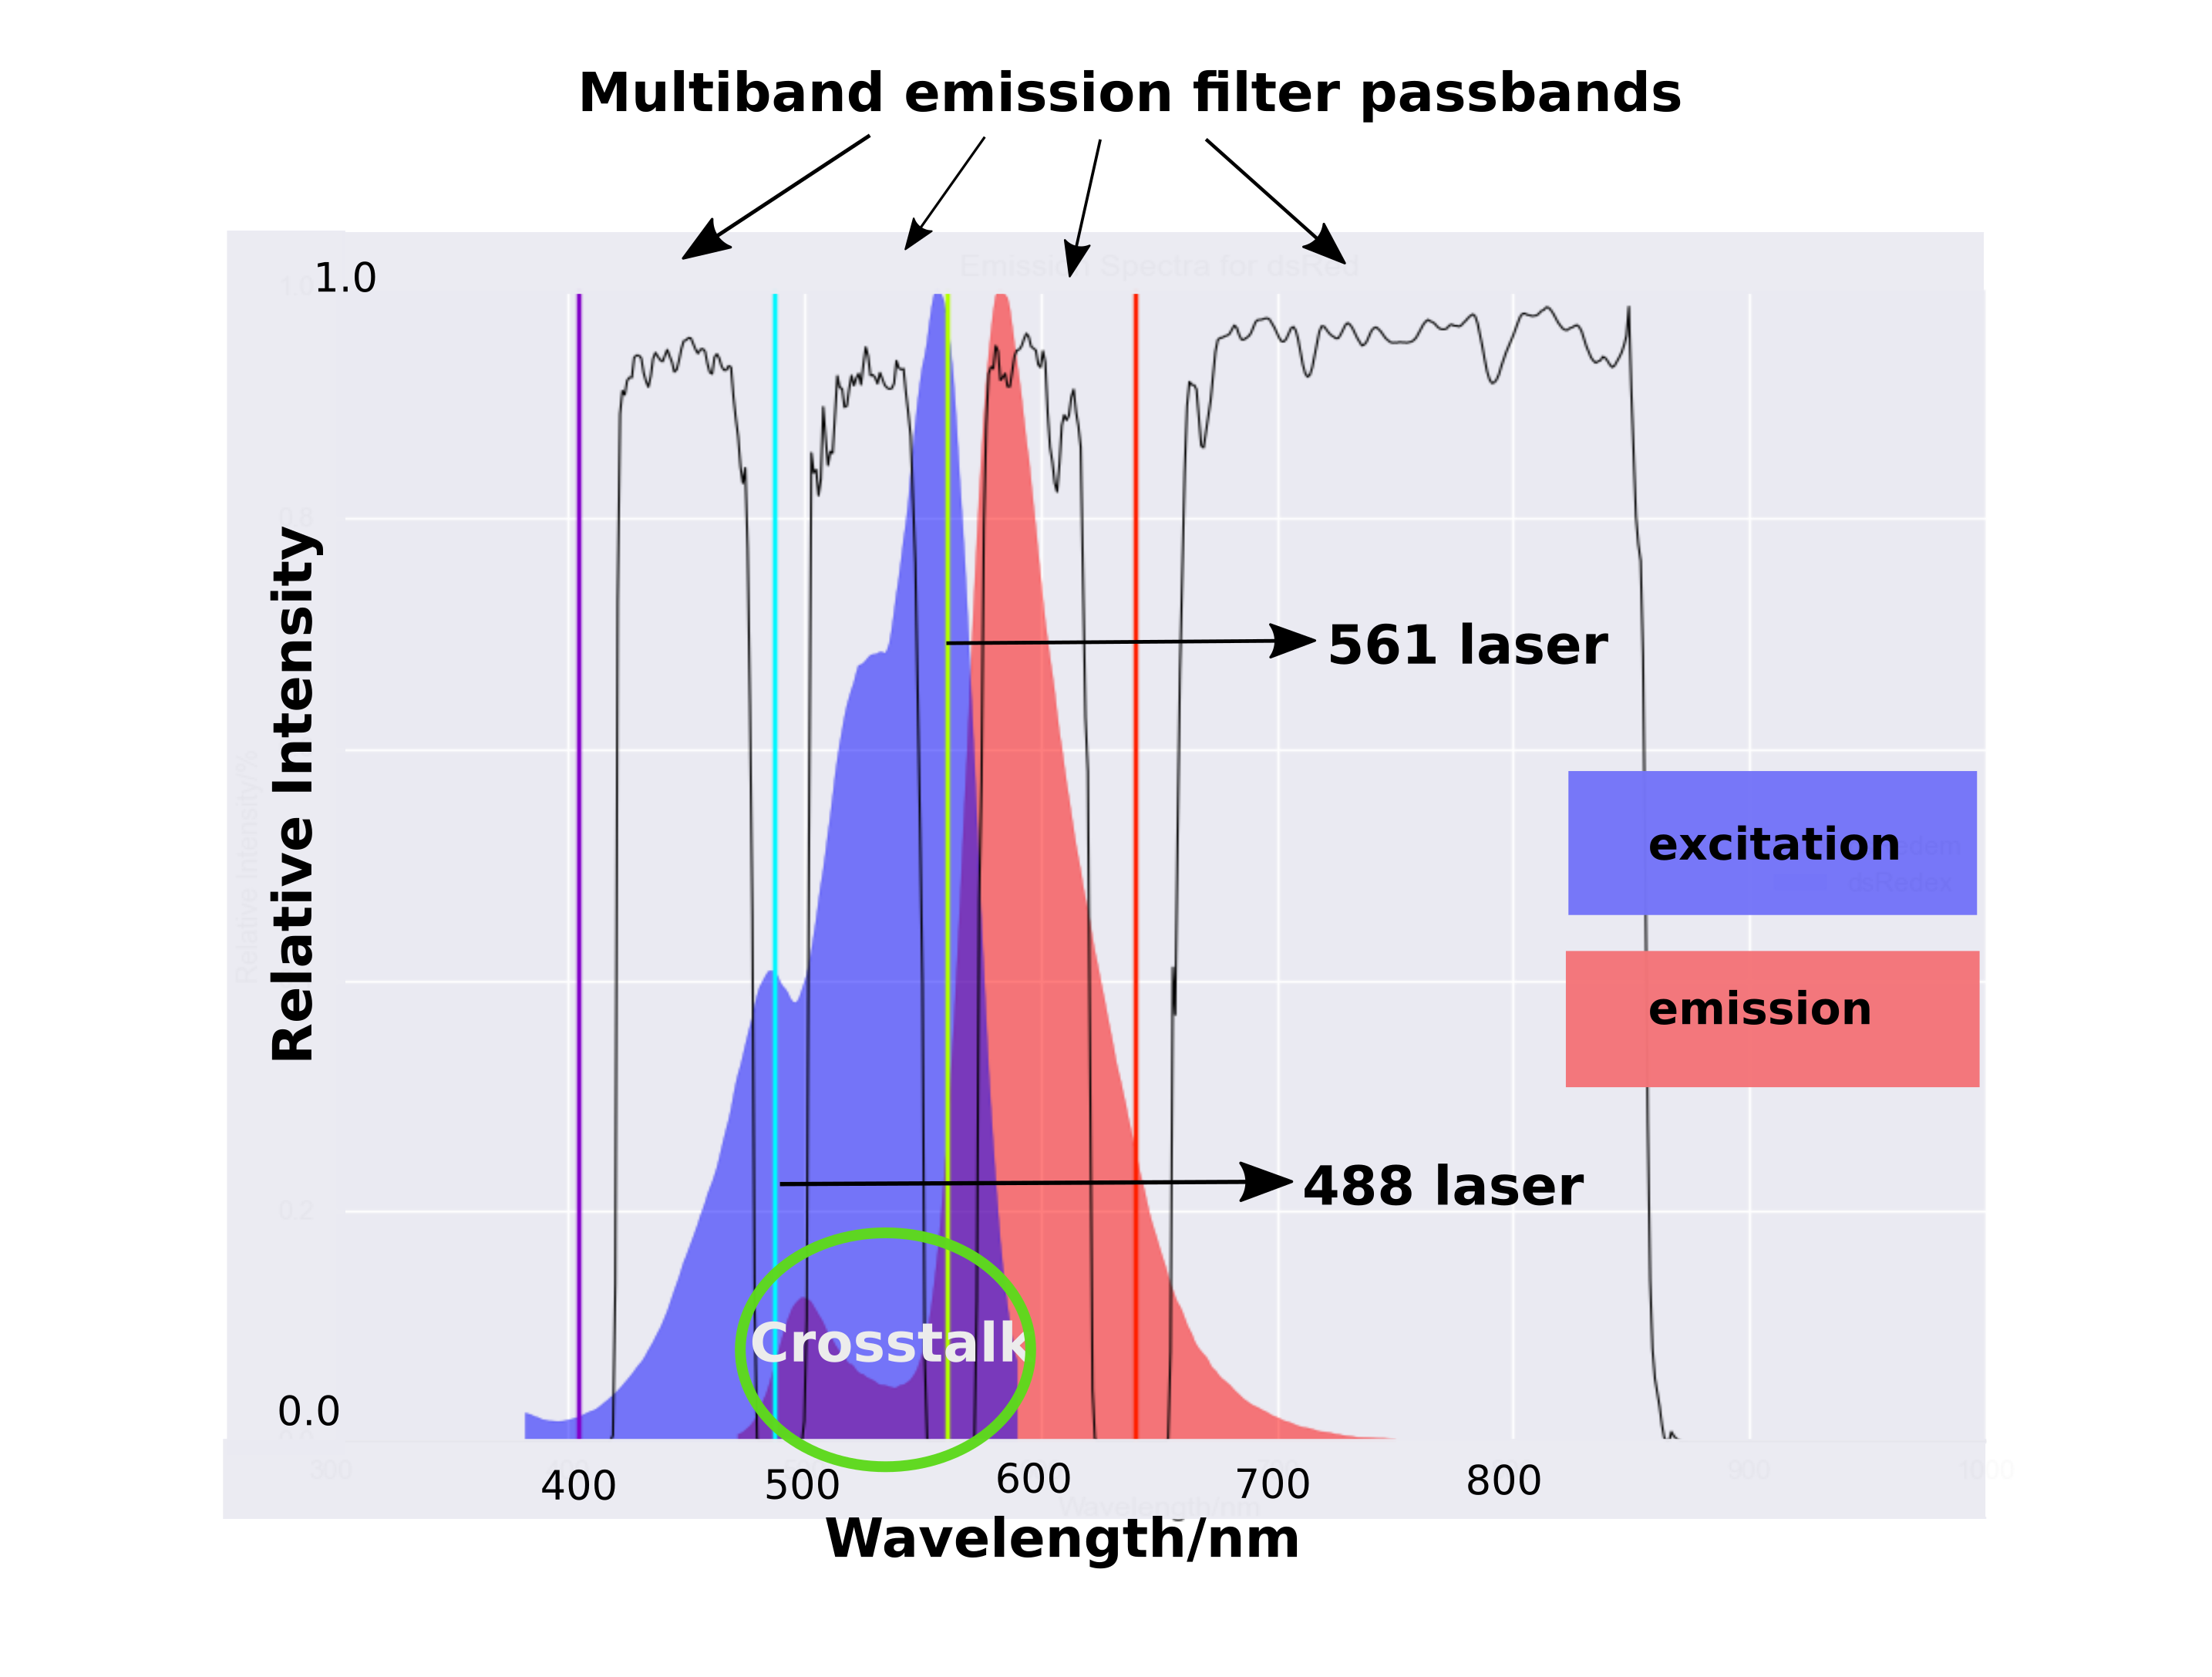
\includegraphics[width=\textwidth]{spectra}
    \caption[Excitation-emission spectra of dsRed mitochondrial matrix marker]{Excitation-emission spectra of dsRed (561nm peak excitation) showing significant region of emission crosstalk from GFP excitation (488nm).}\label{fig:spectra}
\end{figure}
%
This resulted in significant channel crosstalk from the dsRed protein when imaging in the GFP channel (\Fref{fig:xtalk}). To overcome this, the plasmid pFA6a-yomRuby2-Kan (gift of Kurt Thorn, UCSF \cite{lee_improved_2013}) expressing a yeast codon optimized deep red fluorescent protein (mRuby2) was PCR amplified with primer sequences \texttt{\seqsplit{ 5$'$ACAGCGGGTACCATGGTGTCCAAAGGAGAGGAGTTAATC$'$3}} and \texttt{\seqsplit{ 5$'$ACAGCGCTCGAGCCTTACTTATACAATTCATCCATACCACCGC$'$3}} (\Fref{fig:plasA}). The insert was cloned into a matrix targeting plasmid, pVT-100UGFP2 (gift from Jodi Nunnari, UC Davis \cite{meeusen_mitochondrial_2004}), at the XhoI and Kpn restriction sites \Fref{fig:plasB}. Colonies of this new strain (SRY-124, background strain W303a) expressing this new plasmid, pVT100-mRuby2 (URA) were verified by digestion at the EcoRI and HindIII + SphI site (\Fref{fig:plasC}).
%
\begin{figure}[htp]
	\centering
    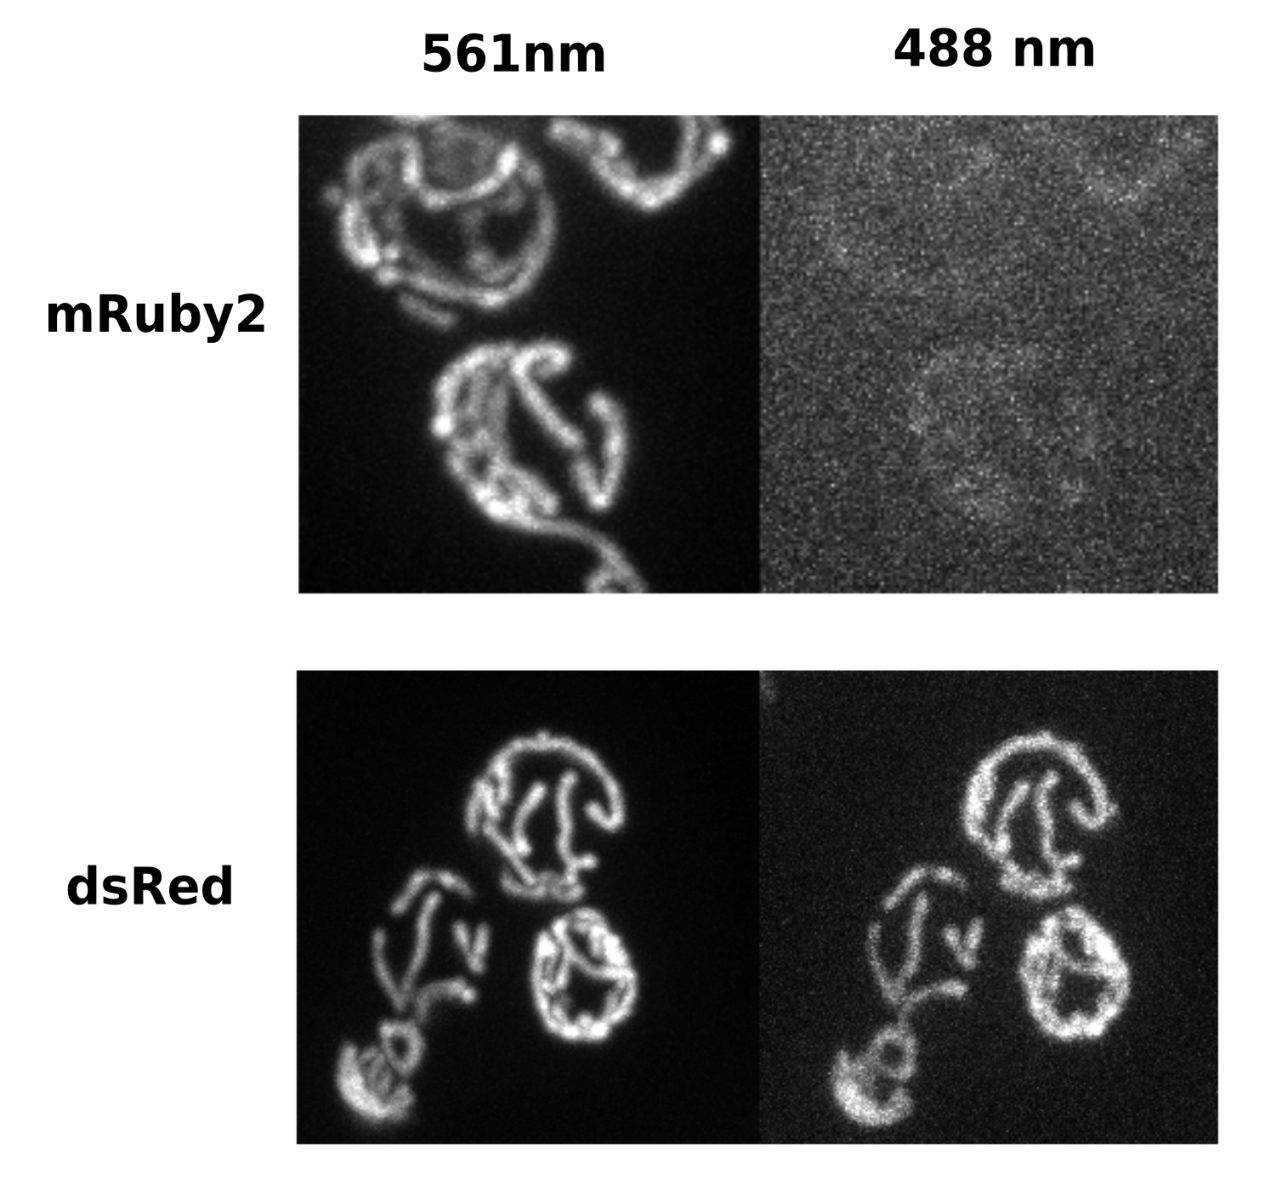
\includegraphics[width=\textwidth]{b4after}
    \caption[Comparison of crosstalk levels in mRuby2 and dsRed.]{Comparison of crosstalk levels in mRuby2 and dsRed.\\
    Shown in this figure are cells expressing either mRuby2 or dsRed and imaged at 561nm and 488nm. The optimum excitation frequency for these proteins are at 561nm, but significant crosstalk is apparent in dsRed when excited at 488nm. Theoretically with zero crosstalk there is zero signal in the 488nm channel, but the intensity of the 488nm channel was 20\% of the value in the 561nm channel. This percentage (and hence crosstalk level) was significantly reduced in mRuby2 (488nm intensity was 3\% of the 561nm channel).}\label{fig:xtalk}
\end{figure}
% 
\begin{figure}[htp]
	\centering
    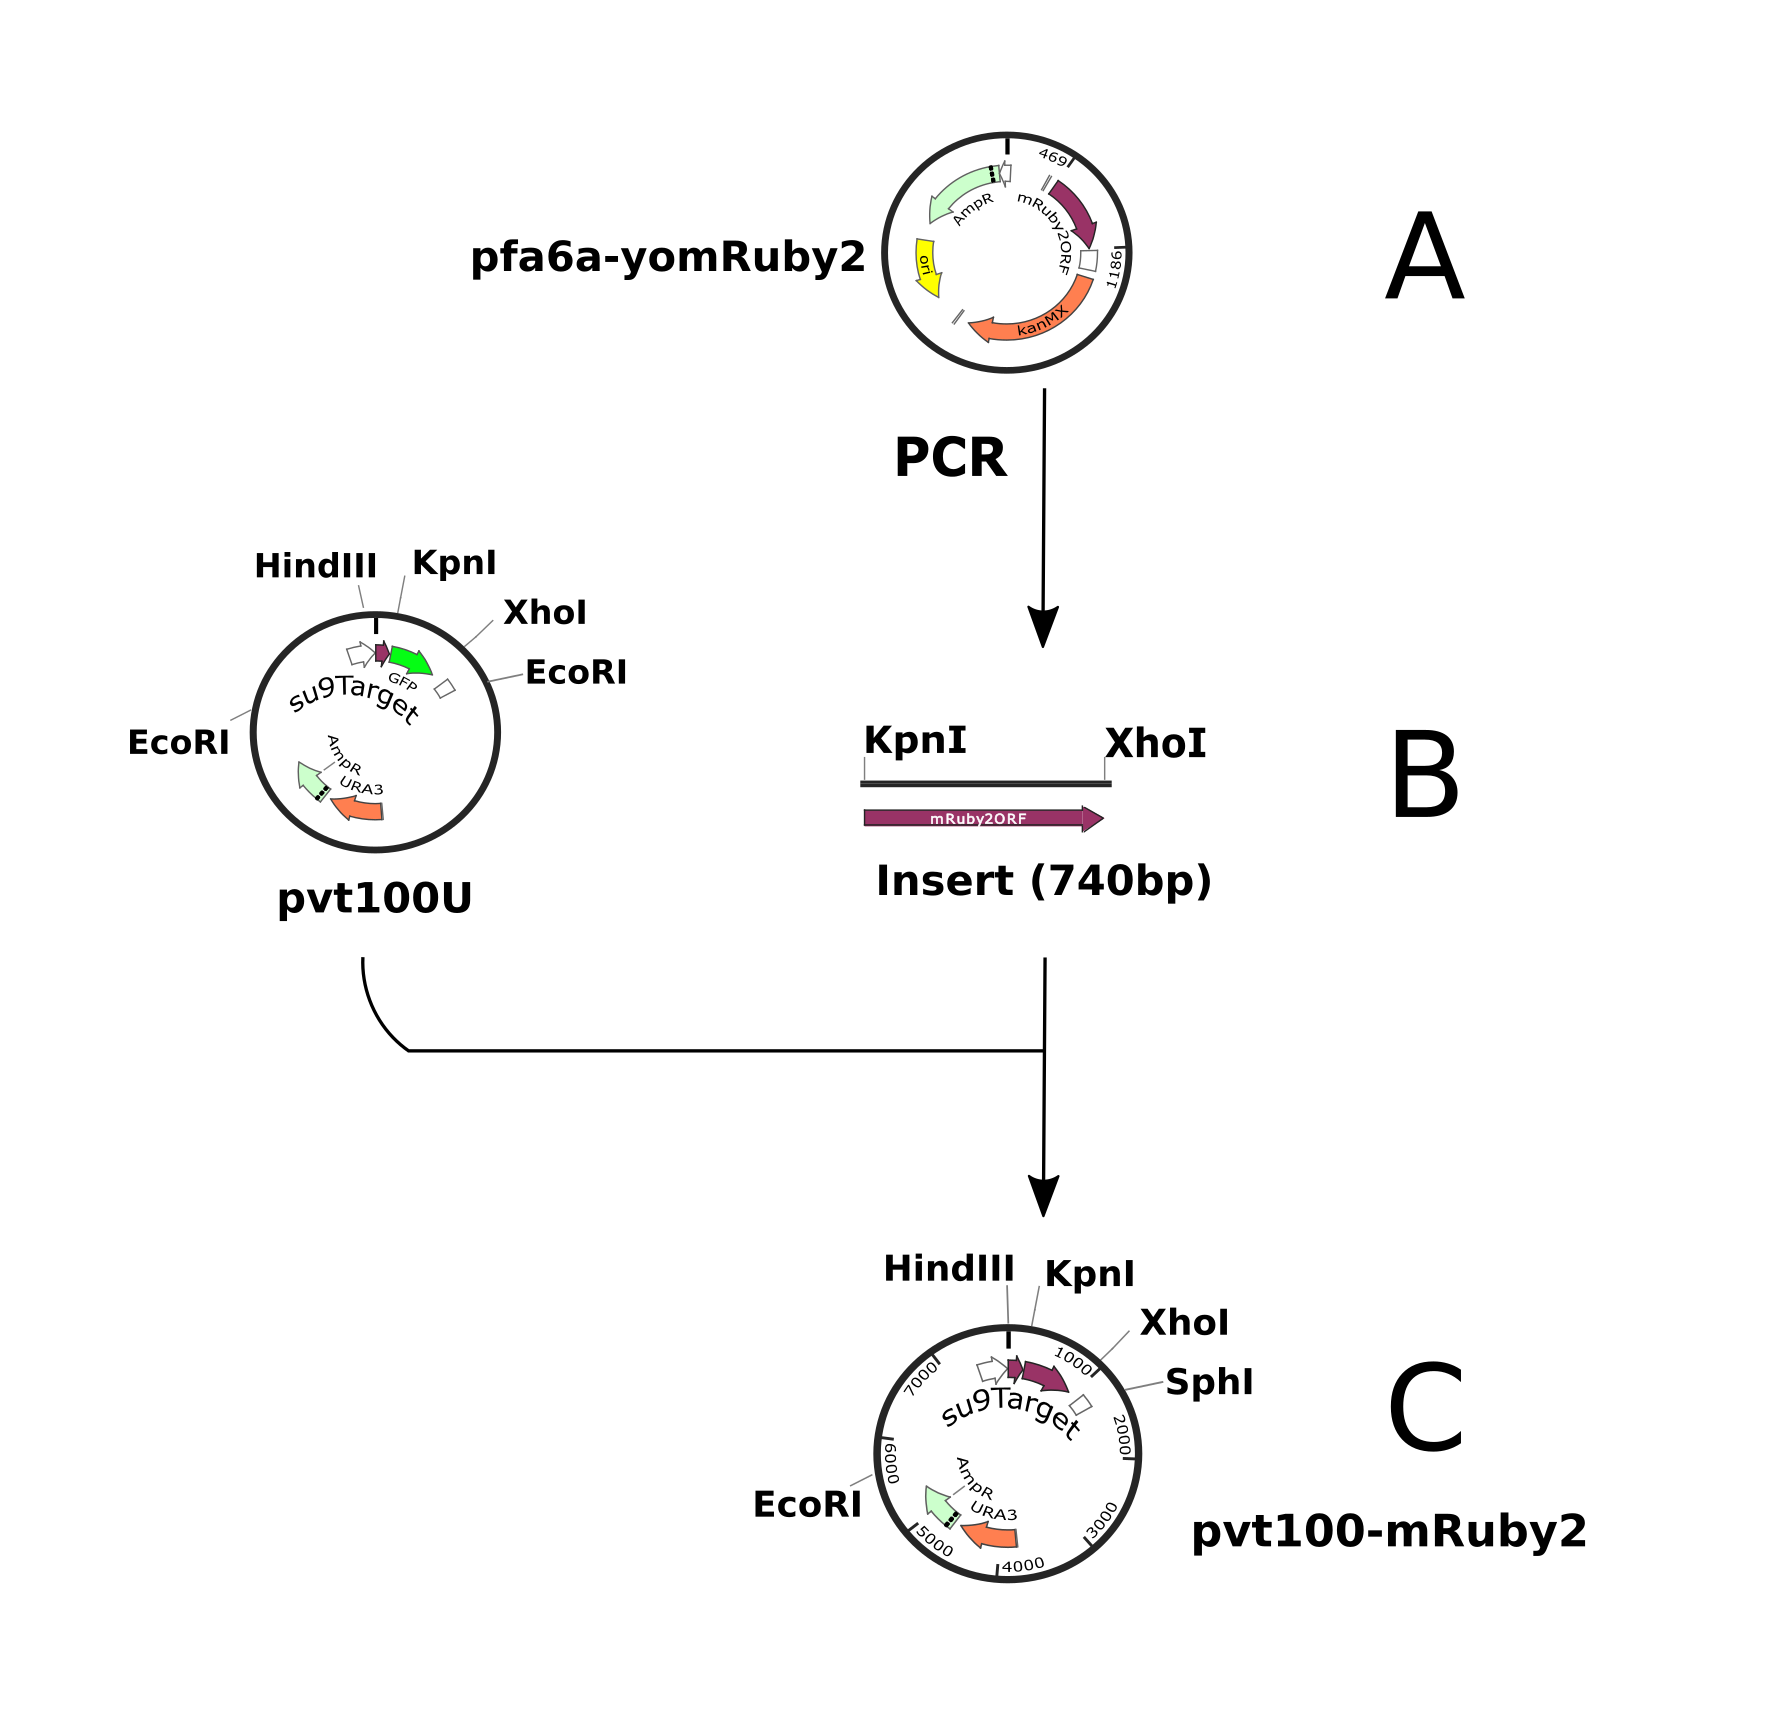
\includegraphics[width=\textwidth]{plasmid}
        \subcaptionbox{Original plasmid (gift of Kurt Thorn, UCSF) containing the mRuby2 sequence.\label{fig:plasA}}[\linewidth]{}
		\subcaptionbox{Insert was generated by PCR amplification of mRuby2 sequence at the KpnI and XhoI restriction sites and cloned into pvt100U-GFP2 (gift of Jody Nunnari, UC Davis).\\Primer sequences for the insert were \texttt{\seqsplit{5$'$ACAGCGGGTACCATGGTGTCCAAAGGAGAGGAGTTAATC$'$3}} and \texttt{\seqsplit{5$'$ACAGCGCTCGAGCCTTACTTATACAATTCATCCATACCACCGC$'$3}}.\label{fig:plasB}}[\linewidth]{}
		\subcaptionbox{The new plasmid, pvt100-mRuby2 (URA) was cloned into W303a background strain and the new strain was SRY-124. The plasmid was verified for correct insertion by digestion at the HindIII and SphI site.\label{fig:plasC}}[\linewidth]{}
		\caption{Plasmid construction details for pvt100-mRuby2 for cloning into SRY-124.\label{fig:plasmid}}
    \end{figure}
%
This new strain exhibited significantly reduced crosstalk from the mRuby2 fluorescent protein when imaging in the GFP region, which is where the functional reporter DiOC$_6$ operates in (\Fref{fig:xtalk}). On average the amount of crosstalk was reduced from an average of about 20\% using dsRed to less than 3\% when using mRuby2.
\subsection{Cell preparation and loading of functional dye}\label{sec:loaddye}
 Cells from strain SRY-124 (described in \fref{sec:strain}) were inoculated from -URA selection plates and cultured overnight at 30°C in a roller drum in the growth media of interest (Yeast Extract + Peptone + either 2\% glucose (YPD), 2\% glycerol+ 2\% ethanol (YPE), 2\% lactate (YPL) or 2\% raffinose (YPR)). A 5 ml 0.05 OD dilution from this overnight culture (which was at \textasciitilde{0.5} OD$_{600}$) was grown to mid-log phase (0.4--0.5 OD$_{600}$). Samples were pipetted out into a 1.5 ml microcentrifuge tube and diluted down in growth media to a ratio of 1:8 before been vortexed briefly to break up cell clumps. 
The cells were stained with DiOC$_6$ (D-273, Thermo Fisher) to a final concentration of \SI{100}{\nmol} from an original master stock concentration of \SI{10}{\umol} (in ethanol). The loaded cells were incubated for 30 minutes at 30°C, spun and wash before reloading in fresh growth media with \SI{100}{\nmol} of DiOC$_6$.

A glass bottom 96 well plate was treated with 1\% Glassclad18 (Gelest Inc, PA) for 5 minutes and oven dried at 70°C overnight. Glassclad18 is a monomeric octadecylsilane glass surface coating that imparts a negative charge to the surface. This ensures that the DiOC$_6$ dye does not bind to the glass, which would result in a high background and reduce the signal to noise ratio from the mitochondria (\Fref{fig:glas18}). Subsequent to surface treatment, each well was loaded with \SI{100}{\ul} of Concanavalin-A (C-5275, Sigma Aldrich) to help cell adhesion to the glass surface. Each well was then loaded with \SI{100}{\ul} of growth media containing cells stained with DiOC$_6$ (D-273, Thermo Fisher) and allowed to incubate at 30°C for about 15 minutes to allow the cells to adhere to the glass surface. The remaining cells in the solution were aspirated and \SI{200}{\ul} of fresh growth media containing \SI{100}{\nmol} of DiOC$_6$ was loaded into the well and immediately imaged.

%
\begin{figure}[htp]
	\centering
    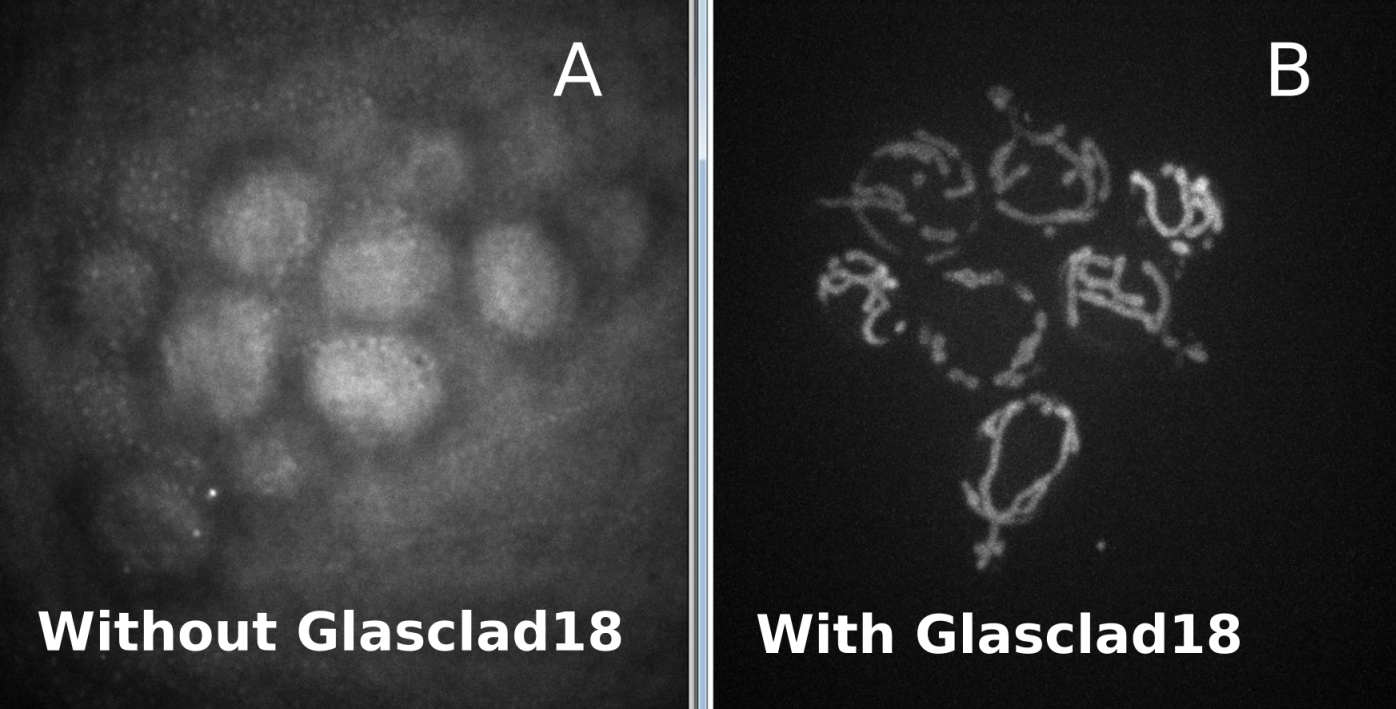
\includegraphics[width=.85\textwidth]{glas18}
    \subcaptionbox{Maximum intensity projection of a cluster of W303a cells stained with DiOC$_6$ loaded in a glass bottom 96 well plate. The dye adheres to the glass surface, causing a significant background image that washes out the signal from mitochondria stained with the dye.\label{fig:glasA}}[\linewidth]{}
    \subcaptionbox{Maximum intensity projection of a cluster of cells loaded on a well treated with Glasclad18. There is significant improvement in the signal to background noise ratio, enabling the mitochondria stained with DiOC$_6$ to be clearly visible.\label{fig:glasB}}[\linewidth]{}
    \caption[Glas18 surface treatment to improve signal to noise ratio]{Signal to noise ratio improvement from DiOC$_6$ channel (mitochondrial membrane potential (ΔΨ) marker) after application of Glasclad18 on imaging surface.}\label{fig:glas18}
\end{figure}
%
\subsection{Image microscopy pipeline}
The cells that were stained and loaded into the 96 well plate in \fref{sec:loaddye} were immediately transferred to the microscope stage holder with the housing chamber set at 30°C. Each well contained cells growing in different carbon types and were imaged as follows:
\begin{enumerate}[label=\arabic*), leftmargin=*, itemindent=0pc]
\item A field of stationary, non clumped cells expressing the fluorescent protein (mRuby2) adequately with healthy mitochondrial morphology was selected via the eyepiece. Individual cells for imaging were then selected via the camera from a region adjacent to this field.
\item Excitation laser power was selected to the minimum needed to give a good signal to background intensity ratio. The minimum signal over background fluorescence was 1.16 (typical background noise \textasciitilde{2000}, minimum signal \textasciitilde{2400}) for accurate skeletonization by MitoGraph v2.0. Photo-damage of the mitochondria was avoided by using low laser power for each channel (typically no more than 20\% of the max range of the laser). Cells with medium to low expression of the protein were selected in order to minimize crosstalk between the signals from the fluorescent protein and the mitochondrial membrane potential dye. This also avoided aberrant mitochondrial morphology due to over expression of the protein in the mitochondria. Typical intensity values for cells were between 3000 – 5000 a.u.
\item A Z-stack was taken of the cells in order to generate a 3D rendering of the mitochondrial network within the cell. The filter settings were set to the appropriate excitation and emission wavelength of the fluorescent protein being expressed. The bottom and top slice positions were set so that the mitochondria was just slightly out of focus at these positions to ensure that the entire mitochondrial network in the cell was imaged.
\item Exposure time was set at 100 ms to reduce photo damage and minimize organelle movement during z-stack image acquisition. Each channel was switched sequentially by the AOTF before moving to the next z-position to minimize organelle movement between channels (\Fref{fig:zstack}). All hardware controls (stage movement in the z-direction during z-stack acquisition and AOTF laser switching) were triggered via TTL which ensured minimum hardware latency.
\end{enumerate}
%
\begin{figure}[htp]
	\centering
    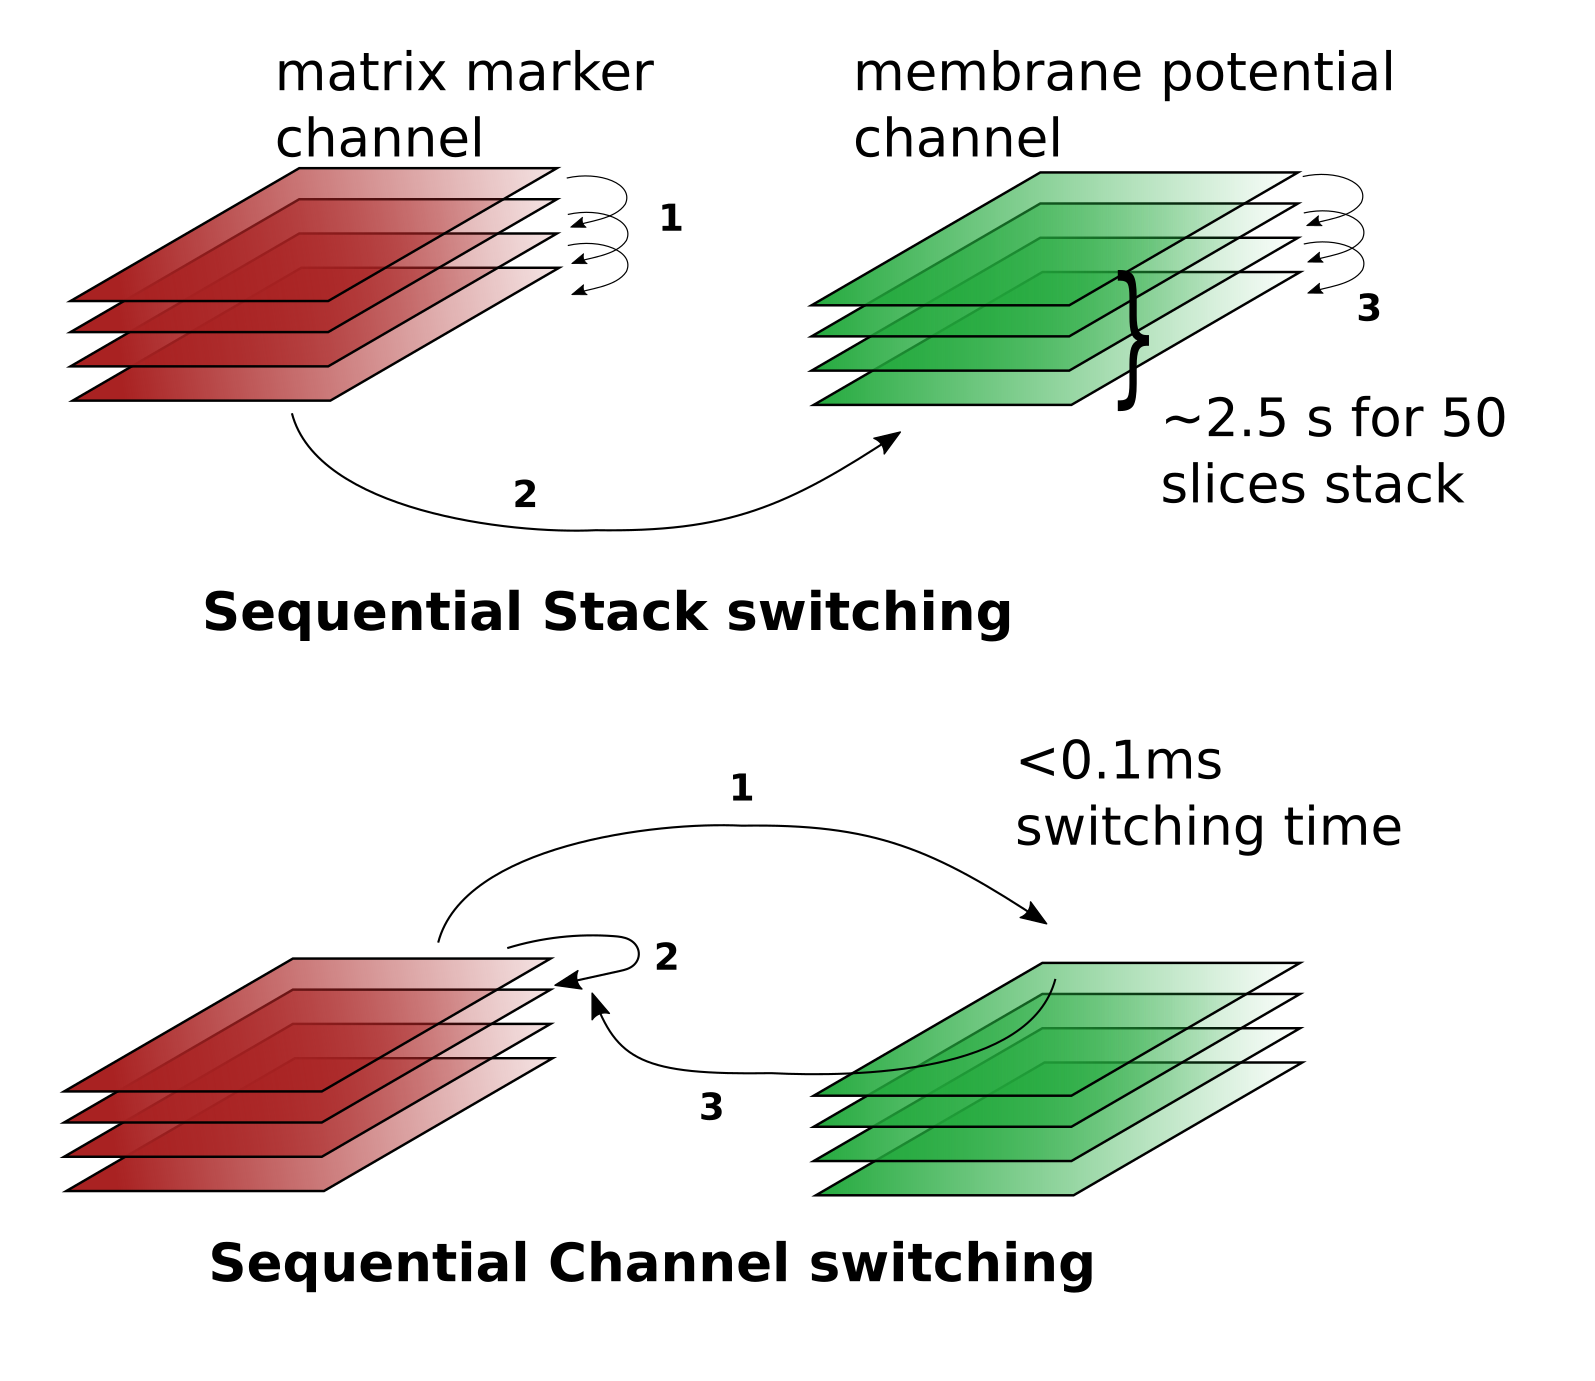
\includegraphics[width=.85\textwidth]{zstack}
    \caption[Comparison of sequential channel vs sequential stack switching scheme.]{Comparison of sequential channel vs sequential stack switching scheme.\\Fast switching time in the sequential channel switching scheme using the AOTF (<0.1ms) ensured that the membrane potential and mitochondrial matrix structural reporting channels (DiOC$_6$ and mRuby2 respectively) were optimally colocalized and did not suffer from organelle movement when compared to the slower sequential stack switching scheme, which typically takes \textasciitilde{2.5} seconds to complete a full stack acquisition.}\label{fig:zstack}
\end{figure}
%
\subsection{Data preparation before input into pipeline}\label{sec:ROI}
Images were saved as 16-bit TIFF stack files. A maximum intensity projection of each Z-stack image was generated automatically via ImageJ batch script. For each cell, the slice with the best focus (defined as where the outlines of the cells in the brightfield stack were least visible) was used to determine if a cell was a budding cell or two individual cells. A region of interest (ROI) was traced out by hand in ImageJ in the corresponding fluorescent image stack (\Fref{fig:budA}). These ROI's were used to crop out the individual cell from the original stack. The cropped out fluorescent channel cell stack was then processed by MitoGraph v2.0 segmentation software. In order to enable cell size measurements, another pair of ROIs were traced (in the brightfield channel) over the mom and bud of the cell and an ellipse fitted to the ROIs (\Fref{fig:budB})
%
\begin{figure}[htp]
	\centering
    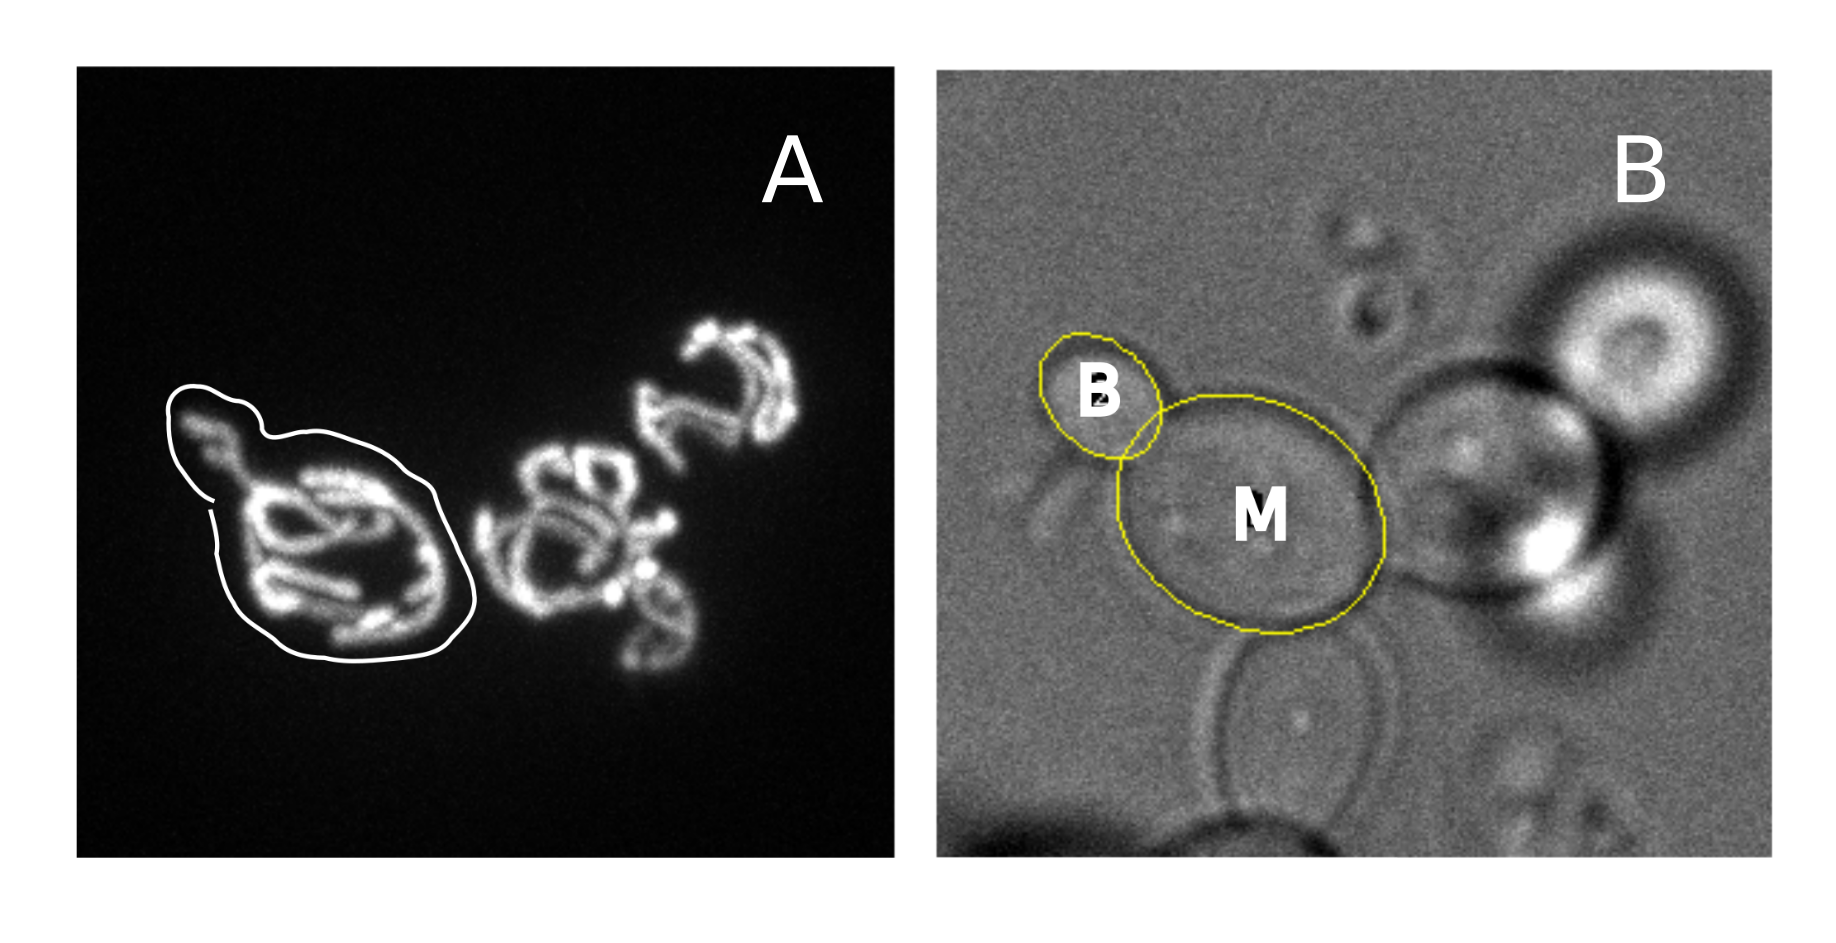
\includegraphics[width=\textwidth]{budtracing}
    \subcaptionbox{Maximum intensity projection of the matrix marker image stack. An ROI (white outline) is hand traced and made into a cropping mask which is applied to the image stack. This cropped image stack was used as input into MitoGraph v2.0 software.\label{fig:budA}}[\linewidth]{}
    \subcaptionbox{Brightfield image of the same cell. In order to enable size measurement of the mom (M) and bud (B) cell, a pair of ROIs were traced and an ellipse fitted over the trace.  \label{fig:budB}}[\linewidth]{}
    \caption{ROI tracing for a budding yeast cell.}\label{fig:budtrace}
\end{figure}
%
\subsection{Artifacts that may arise when mapping ΔΨ to mitochondrial network}\label{sec:artifacts}
 Mapping of ΔΨ to mitochondrial structure is fraught with the potential for artifacts generating a biased or unreliable reading of ΔΨ. These artifacts result from several issues that are related to dye quenching and toxicity, focal plane variation, cell to cell uptake variability and volume variation dependence of fluorescence intensity.
 
While DiOC$_6$ has been long been used as a membrane potential indicator in yeast \cite{hughes_early_2012,john_r._pringle_chapter_1989,koning_dioc6_1993}, most of the other studies mapping function to structure in live mammalian cells tended to use Tetramethylrhodamine (TMRM), the ester form TMRE or the ratiometric dye JC-1. JC-1 is known to have aggregation artifacts and so was avoided. TMRM and TMRE are generally considered less toxic to the respiratory chain compared to DiOC$_6$ and is supposed to have better resistance to self quenching of the fluorophore. However we could not find any discernible impairment of the mitochondria in our hands or in the literature that have also used DiOC$_6$.We found that TMRM could not provide a high enough signal to be successfully mapped to the network, most likely because of the cell wall in yeast that is not present in mammalian cells. Therefore we switched to DiOC$_6$, using the same concentrations, loading protocols and uncoupling tests of other studies that have also used DiOC$_6$ to label ΔΨ \cite{bouillaud_sequence_1994,pena_use_1984,petit_discrimination_1996}. We also verified that at the concentrations we used (\SI{100}{\nmol}), the dye was not operating in quench mode (i.e. could indicate ΔΨ with a higher signal) by observing a higher ΔΨ level in cells that were known to have a high ΔΨ level (respiration) and could be depolarized by an uncoupler (\Fref{fig:fccp}, courtesy of V.Jayashankar).

The intensity of the mitochondrial membrane potential marker and the matrix marker is strongly affected by their position \cite{gerstenberger_heterogeneity_2012,wikstrom_-cell_2007} in the focal plane due to spherical aberration effects that originate from refractive index mismatch. Refractive index mismatch is inevitable when one uses an oil immersion objective to image live cells. This results in a distorted point spread function that causes regions of the cells that are far away from the cover slip to have the lowest signal intensity.

Variation in dye intensity can also result from differences in dye uptake levels between cells. This means that we cannot convert raw intensity values of the ΔΨ channel into absolute voltage to compare ΔΨ between cells, as we cannot control for dye uptake issues that are independent of ΔΨ. This is the disadvantage of using a dye to label ΔΨ, however we can still quantify ΔΨ distributions within a cell as there should be not any variability in dye uptake within the same cell that are not related to ΔΨ.

The last issue relates to intensity variation of the fluorophore due to volume changes. This applies more to the case of the mitochondrial structural marker. Although the expression of the matrix targeted fluorescent protein is not dependent on membrane potential, volume variation along a tubule can result in a thick section of tubule having a higher integrated intensity compared to a thin tubule. 
\subsection{Pipeline to map ΔΨ to mitochondrial network with normalization and scaling to control artifacts}
Having listed all the artifacts that can arise when mapping function to structure, the next step is to account for these artifacts and controlling for their effects where possible when we map function to structure. The first step of the pipeline is a background subtraction of the two channels to correct for camera offset. The background value was set by picking two points without any signal in the original stack. For each channel, a spherical region 2.5 pixels in radius (equivalent to \SI{138}{\nm}) was set along every point coordinate ($x_i,y_i,z_i$) of the skeleton generated by MitoGraph v2.0. A point cloud from this sphere was mapped onto the 3D voxels file of each channel. A mean value of all the points lying within this point cloud was assigned to the point ($x_i,y_i,z_i$).  This averaging served as a smoothing filter to correct for noise/jitter in the channel while reasonably capturing the signals from a typical mitochondrial tubule with thickness \textasciitilde{\SI{300}{\nm}} \cite{egner_fast_2002}.

For the mitochondrial matrix marker, the values were then normalized to 0 and 1 by scaling to the min and max of the channel in that particular cell. This means that the matrix channel was scaled to the intensity of the narrowest portion of the tubule in that cell's mitochondrial network. This controls for the matrix intensity variation due to tubule thickness variations, hence addressing the problem of volume variation dependence of fluorescent protein intensity.

The background subtracted DiOC$_6$ channel representing membrane potential was then normalized to the matrix channel (scaled to min-max). This normalization controls for the focal plane variation problem as both channels are affected similarly by spherical aberration, thus their ratios 'cancel' out the errors. The resulting channel represents a spatial 'heat map' of mitochondrial membrane potential over the mitochondrial network within that cell. A flowchart of the pipeline is shown (\Fref{fig:pipeline})

The source codes for the pipeline modules are included in Appendix \ref{pipecode}.
%
\begin{figure}
	\centering
    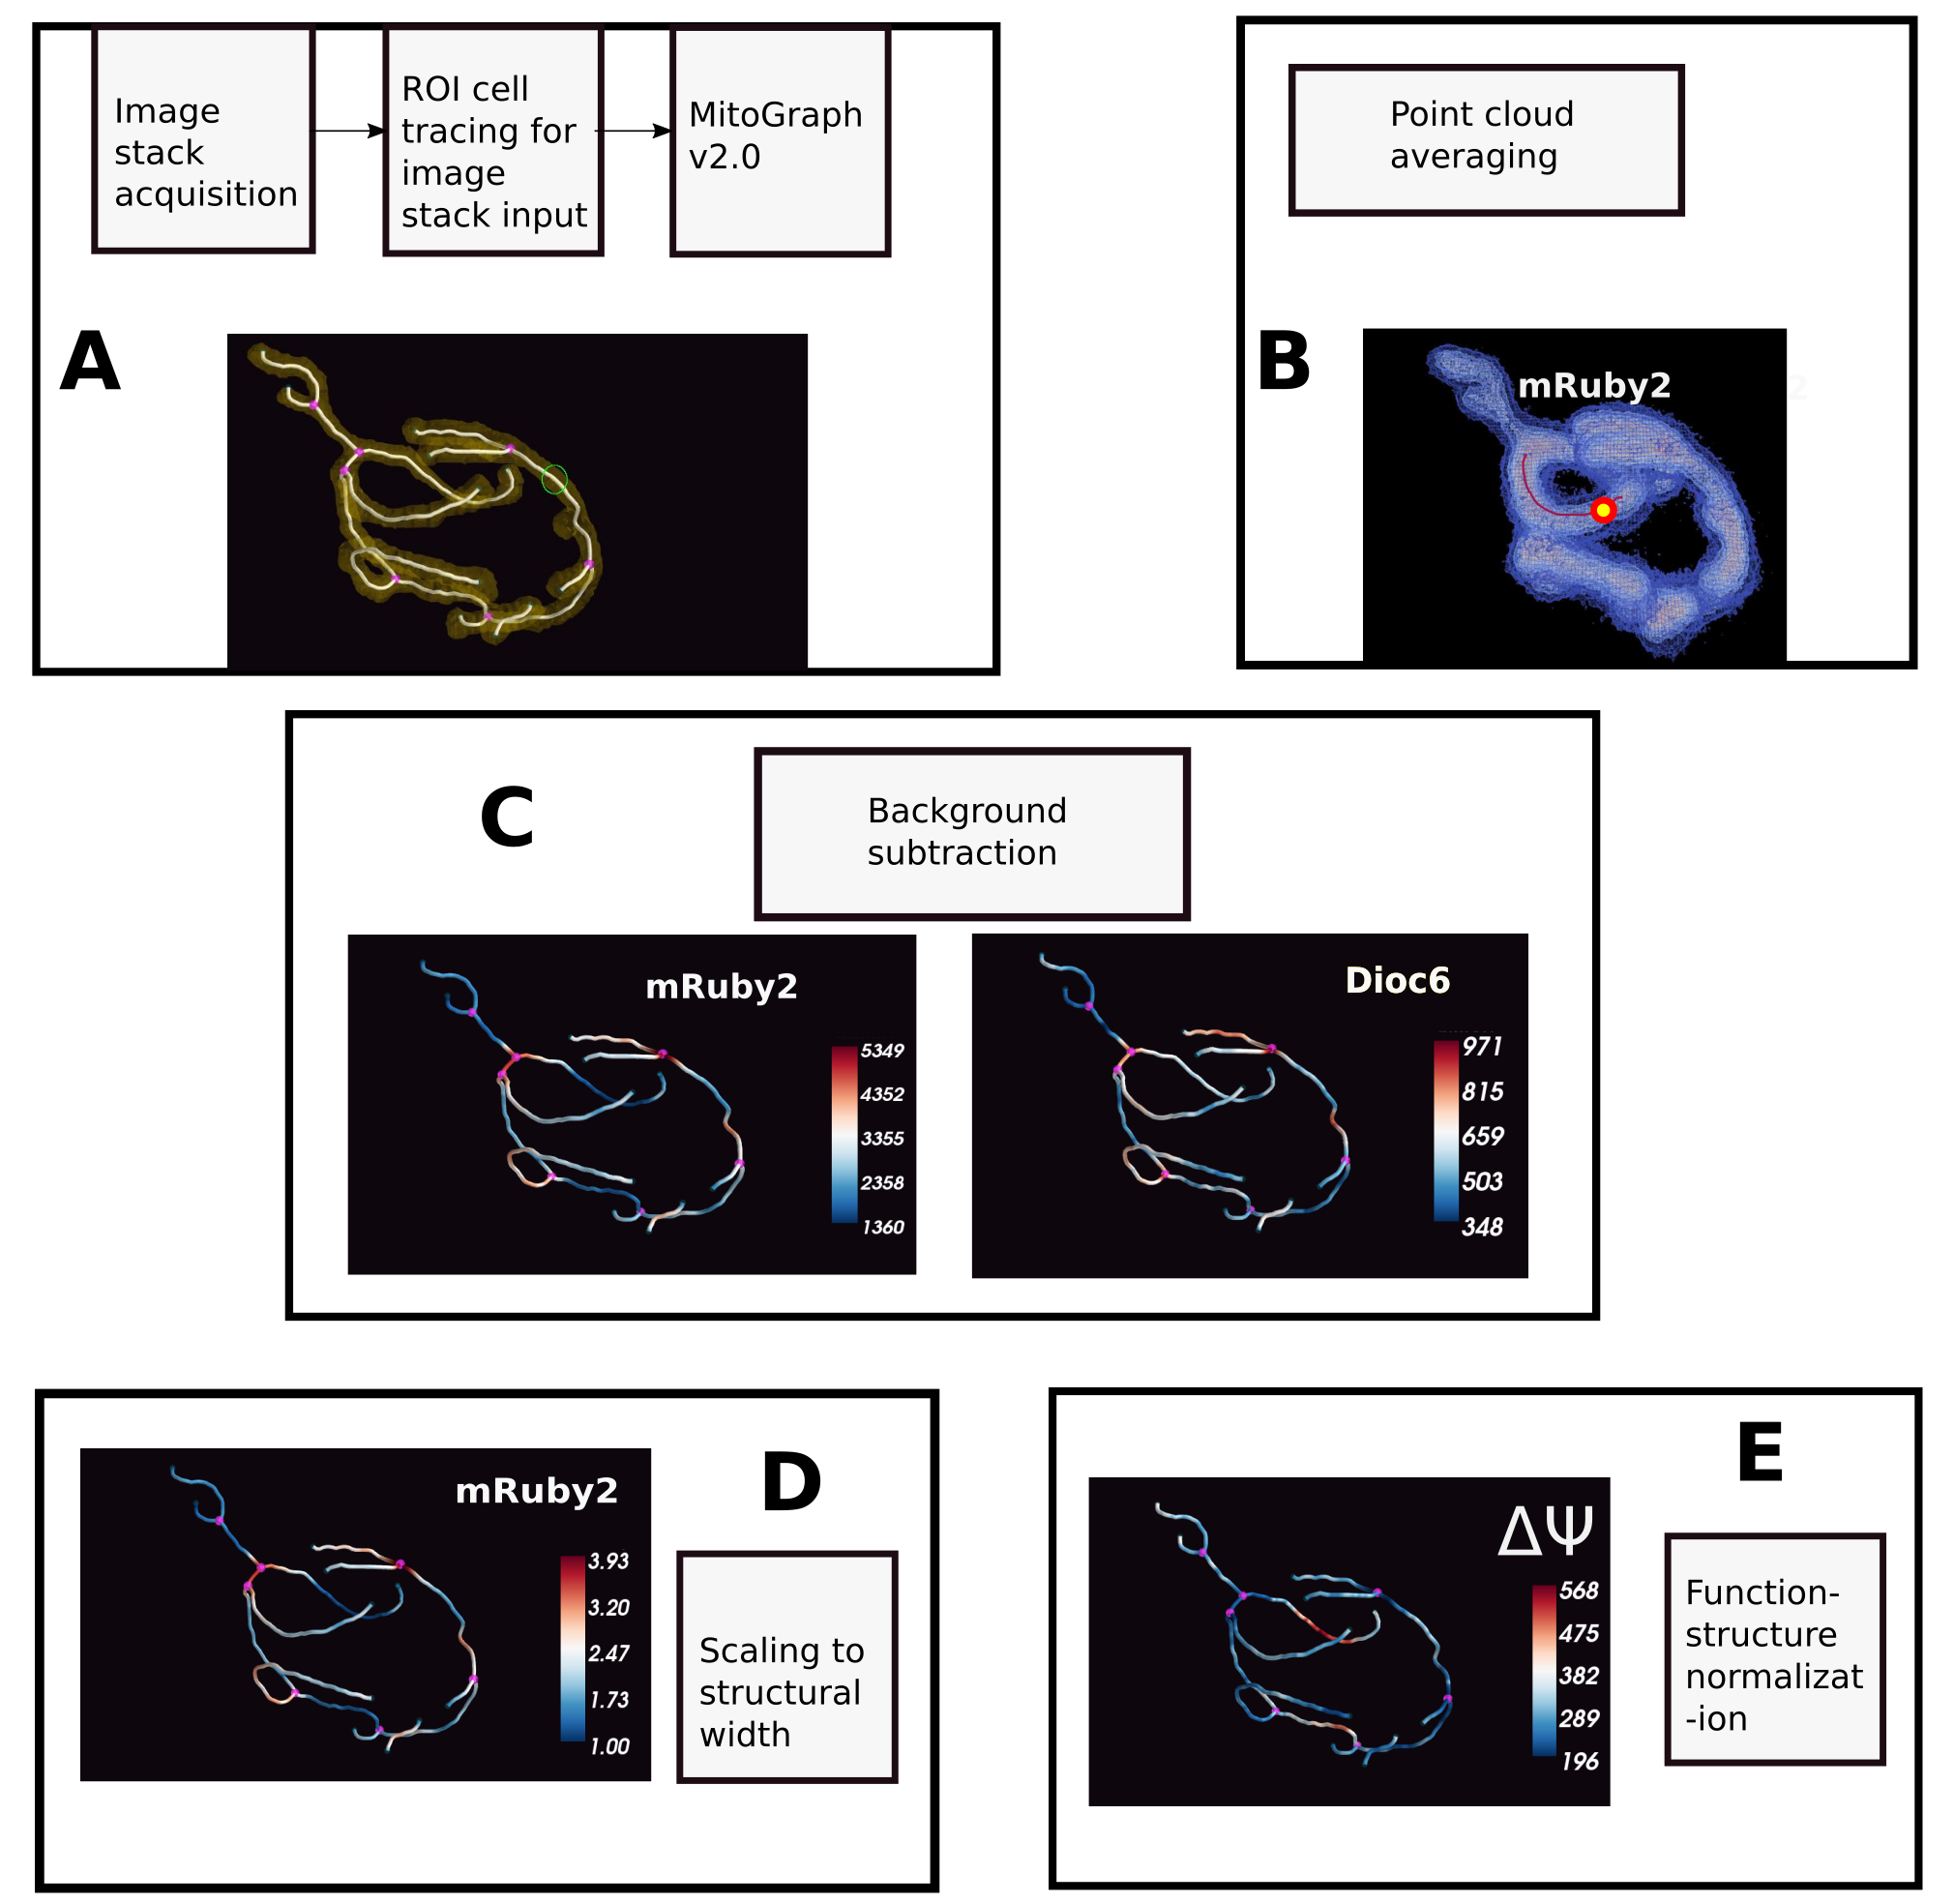
\includegraphics[width=\textwidth]{pipeline}
    \captionof{figure}[Structure-function mapping pipeline]{Pipeline modules for mapping function (ΔΨ) onto structure.\\The boxes A-E roughly correspond to the individual program modules used in the pipeline. Module A represents all steps from image acquisition up to skeletonization by MitoGraph v2.0 to generate a raw skeleton and surface rendering of the matrix marker channel (mRuby2). Module B represents the point cloud averaging from the voxels of the 3D image stack. For each point along the line, the mean intensity value of all points within the red sphere was assigned to the point marked in yellow. Module C represents a background subtraction module that is applied to both matrix marker and ΔΨ channel. The images shown are the skeleton after background subtraction and point cloud averaging for matrix (mRuby2) and ΔΨ (DiOC$_6$). Module D represents a min-max scaling of the pixel intensities to the minimum intensity to control for volume dependence of matrix marker channel due to tubule width variation. Module E represents the spatial heat map of ΔΨ along the skeleton after normalizing the background corrected ΔΨ channel (from module C, DiOC$_6$) with the scaled, background subtracted matrix channel (from module D).}\label{fig:pipeline}
\end{figure}
%
\subsection{Data wrangling – database structure}\label{sec:database}
The raw outputs of MitoGraph v2.0 that are used in the pipeline are a set of coordinates representing a skeleton of the mitochondrial network along with a connectivity list with information on how the points connect to each other. The other outputs that are used are the 16-bit scalar intensity values of each channel for the matrix marker, ΔΨ and tubule width of the mitochondrial network.

The native file format of the data is in the Visualization Toolkit (VTK, \url{http://www.vtk.org/}) format which is a C++ library for 3D scientific visualization with interfaces for Python and other interpreted languages. The native data is 'wrangled' or organized into a standard tidy data form \cite{wickham_tidy_2014} and stored using a database structure with the Pandas data analysis module (\url{http://pandas.pydata.org/}) in Python 2.7. Data wrangling involves reshaping the raw data format structure (i.e. a mitochondrial network) into a form that is most convenient for performing calculations at a scale that is relevant to the type of analysis. The output can then be aggregated if necessary for further calculations downstream or for visual data presentation.

The database (\Fref{fig:database}) incorporates \textasciitilde{100} variables which are measures related to structure and function across multiple size scales as well as measures that relate to either heterogeneity, function or cell asymmetry. These variables were calculated from the outputs of MitoGraph v2.0 as well as other meta-data (for example cell name, cell carbon source) and non MitoGraph v2.0 derived data (such as oxygen consumption rates). The database enables convenient data exploration and multi-scale analysis of structure-function in mitochondrial networks, with the data organized in 'tidy-data' form \cite{wickham_practical_2008} and allowing a layered grammar of graphics presentation of the results \cite{wilkinson_grammar_2005}. A list of variables from the database is included in the Appendix section (\Fref{tab:long}).

The source code for constructing the database is included in Appendix \ref{dbcode}.
\begin{figure}[htp]
	\centering
    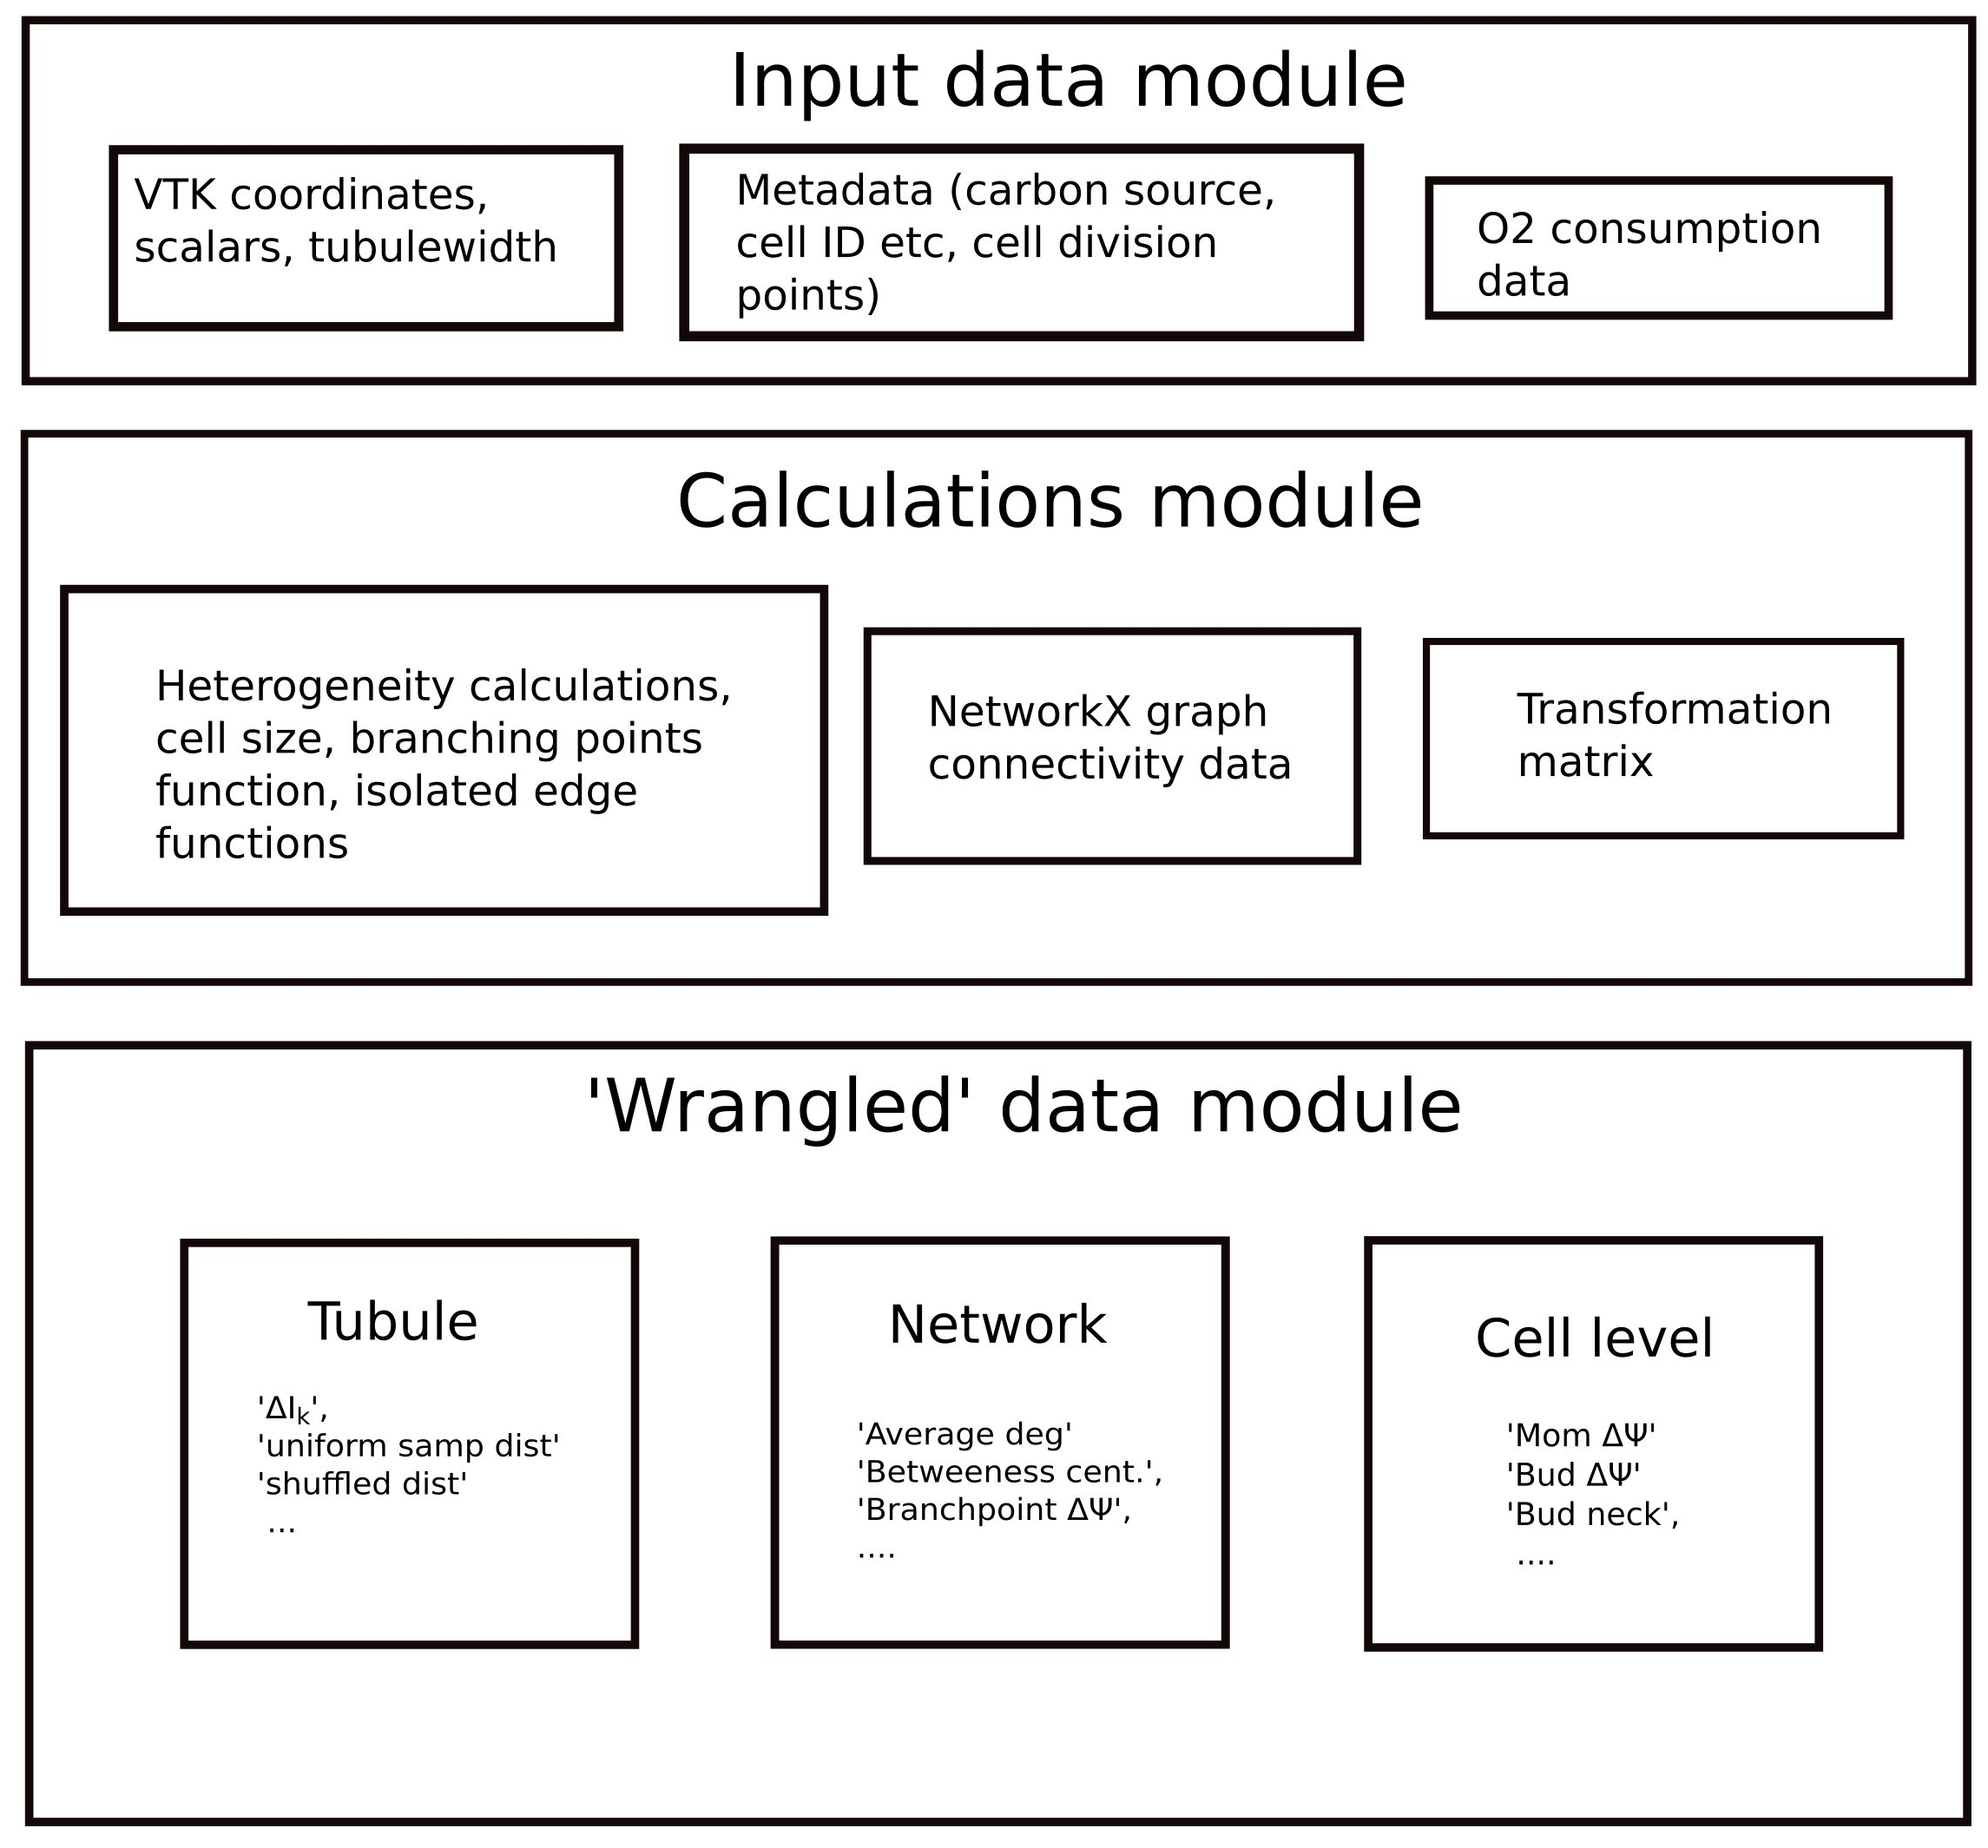
\includegraphics[width=\textwidth]{database}
    \caption[Multi-scale structure-function database]{Schema of database used for multi-scale analysis of structure-function relationship in yeast mitochondrial networks.\\
Shown here is the database used in this thesis which uses the Pandas data analysis module in Python 2.7. The database consists of an input data module, a calculations module and a wrangled data module.
The input data module stores the outputs of MitoGraph v2.0, metadata sources and oxygen consumption data. The primary calculations module processes the data from the input data module to obtain measures such as connectivity, heterogeneity measures and transformation matrix used for calculating mother-daughter cell axis. The processed data is then reshaped and aggregated ('wrangled') into the form most appropriate for the scale and functional measure it will be used for, for example in mother-bud functional asymmetry analysis.}\label{fig:database}
\end{figure}